\documentclass{article}
\usepackage{tikz}
\usetikzlibrary{arrows.meta, positioning, shapes.geometric}
\usepackage[utf8]{inputenc}
\usepackage[UTF8]{ctex}
\usepackage{pgfplots}
\pgfplotsset{compat=1.16}
\usetikzlibrary{calc}
\usepackage{amsmath}
\usepackage{amssymb}
\usepackage{array}
\usepackage{booktabs}
\usepackage{physics}
\usepackage{siunitx}
\usepackage{enumitem}
\usepackage{subcaption}
\usepackage{pgfplots}
\pgfplotsset{compat=1.16}
\pgfmathdeclarefunction{Jzero}{1}{%
  \pgfmathparse{
    ( (#1) <= 8 ) ?
      ( 1 - ( (#1)^2 )/4 + ( (#1)^4 )/64
        - ( (#1)^6 )/2304 + ( (#1)^8 )/147456
        - ( (#1)^10 )/14745600 )
      :
      ( sqrt(2/(pi*(#1))) * cos(deg( (#1) - pi/4 )) )
  }%
}
\usepackage[unicode]{hyperref}
\pdfstringdefDisableCommands{%
  \def\pi{pi}%
  \def\Omega{Omega}%
  \def\hat#1{#1}%
  \def\dfrac#1#2{#1/#2}%
  \def\int{\text{∫}}%
}
\usepackage{xeCJK}
\usepackage{bm}
\usepackage{CJKutf8}
\setCJKmainfont{Noto Serif CJK TC}    % 思源宋體繁體版(推薦)
\setCJKsansfont{Microsoft JhengHei}   % 微軟正黑體
\setCJKmonofont{Noto Sans Mono CJK TC}

\begin{document}

從高斯定律的積分形式出發:
\begin{equation}
\oint_{S} \mathbf{E}\cdot d\mathbf{A} \;=\; \frac{q}{\varepsilon_0}.
\end{equation}

考慮一個以點電荷 $q$ 為中心、半徑為 $r$ 的球面作為高斯面。  
由於對稱性,電場必為徑向,且在球面上大小處處相同:
\[
\mathbf{E}(r) = E(r)\,\hat{\mathbf{r}}, 
\qquad
d\mathbf{A} = \hat{\mathbf{r}}\,dA.
\]

因此內積化簡為
\[
\mathbf{E}\cdot d\mathbf{A} = E(r)\,dA,
\]
並可將 $E(r)$ 提到積分號外:
\begin{equation}
\oint_{S} \mathbf{E}\cdot d\mathbf{A} = E(r)\oint_{S} dA.
\end{equation}

球面的總面積為
\[
\oint_{S} dA = 4\pi r^2,
\]
所以得到
\begin{equation}
E(r)\,(4\pi r^2) = \frac{q}{\varepsilon_0}.
\end{equation}

解出電場大小:
\begin{equation}
E(r) = \frac{1}{4\pi\varepsilon_0}\,\frac{q}{r^2}.
\end{equation}

最後加上方向,得點電荷的電場向量式:
\begin{equation}
\mathbf{E}(r) = \frac{1}{4\pi\varepsilon_0}\,\frac{q}{r^2}\,\hat{\mathbf{r}}.
\end{equation}
\section*{1. 球面上的小塊區域}
考慮半徑為 $R$ 的球面,球座標 $(R,\theta,\phi)$ 中:
- $\theta$ 是極角(由 $z$ 軸量下來,$0\le \theta \le \pi$),
- $\phi$ 是方位角($0\le \phi <2\pi$)。

在球面上,若 $\theta$ 增加一小量 $d\theta$,$\phi$ 增加一小量 $d\phi$,就得到一個「球面矩形」的小區塊。

\section*{2. 兩條邊的長度}
\begin{itemize}
  \item \textbf{沿 $\theta$ 方向}:弧長等於半徑乘以角度差
  \[
  \ell_\theta = R\, d\theta.
  \]
  \item \textbf{沿 $\phi$ 方向}:此時圓的有效半徑是 $R\sin\theta$,因此
  \[
  \ell_\phi = (R\sin\theta)\, d\phi.
  \]
\end{itemize}

\section*{3. 小面積近似}
該小區塊的面積近似為兩邊長相乘:
\[
dA \approx \ell_\theta \cdot \ell_\phi
= (R\, d\theta)\,(R\sin\theta\, d\phi).
\]

\section*{4. 結果}
因此球面面積元素為
\[
\boxed{\,dA = R^2 \sin\theta \, d\theta \, d\phi\, }.
\]

\section*{5. 幾何直覺}
\begin{itemize}
  \item $R^2$:面積必須與半徑平方成正比;
  \item $\sin\theta$:越靠近極點($\theta\to 0$ 或 $\pi$),
  緯線的半徑變小,球面「東西方向」的寬度縮短。
\end{itemize}
\section*{幾何推導回顧}
在半徑為 $R$ 的球面上,令極角 $\theta$ 與方位角 $\phi$ 各增量 $d\theta$、$d\phi$,
得到一個小「球面矩形」。其兩條邊的弧長為
\[
\ell_\theta = R\,d\theta,\qquad
\ell_\phi = (R\sin\theta)\,d\phi,
\]
故小面積
\[
\boxed{\,dA = R^2 \sin\theta\, d\theta\, d\phi\, }.
\]

\section*{TikZ 圖示}
\begin{center}
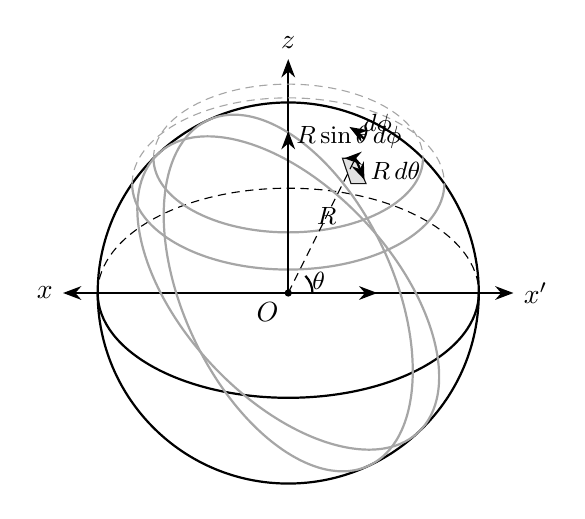
\begin{tikzpicture}[scale=1.1]
  % Parameters
  \def\R{2.2}         % sphere radius (for drawing)
  \def\th{45}         % theta (deg) of the patch center
  \def\dth{10}        % small dtheta (deg)
  \def\ph{25}         % phi (deg) center
  \def\dph{18}        % small dphi (deg)

  % Styles
  \tikzset{
    axis/.style={thick,->,>=Stealth},
    patch/.style={fill=gray!25,draw=black,opacity=0.9},
    arcarr/.style={-{Stealth[length=2.2mm]},thick},
    label/.style={font=\small}
  }

  % Coordinate axes
  \draw[axis] (0,0) -- (0,2.7) node[above] {$z$};
  \draw[axis] (0,0) -- (-2.6,0) node[left] {$x$};
  \draw[axis] (0,0) -- (2.6,0) node[right] {$x'$}; % visual symmetry

  % Sphere (equator as ellipse, meridians as ellipses)
  \draw[thick] (0,0) circle (\R); % outline for visual sphere
  % Equator
  \draw[thick] (-\R,0) arc[start angle=180,end angle=360,x radius=\R,y radius=0.55*\R];
  \draw[densely dashed] (-\R,0) arc[start angle=180,end angle=0,x radius=\R,y radius=0.55*\R];

  % Latitude (theta) circles: show the one at current theta and theta+dtheta
  \pgfmathsetmacro{\rsin}{\R*sin(\th)}
  \pgfmathsetmacro{\rcos}{\R*cos(\th)}
  \pgfmathsetmacro{\rsinUp}{\R*sin(\th+\dth)}
  \pgfmathsetmacro{\rcosUp}{\R*cos(\th+\dth)}

  % Draw the two latitude circles as ellipses at heights z=R*cos(theta)
  \begin{scope}[shift={(0,\rcos)}]
    \draw[thick,gray!70] (-\rsin,0) arc[start angle=180,end angle=360,x radius=\rsin,y radius=0.55*\rsin];
    \draw[densely dashed,gray!70] (-\rsin,0) arc[start angle=180,end angle=0,x radius=\rsin,y radius=0.55*\rsin];
  \end{scope}
  \begin{scope}[shift={(0,\rcosUp)}]
    \draw[thick,gray!70] (-\rsinUp,0) arc[start angle=180,end angle=360,x radius=\rsinUp,y radius=0.55*\rsinUp];
    \draw[densely dashed,gray!70] (-\rsinUp,0) arc[start angle=180,end angle=0,x radius=\rsinUp,y radius=0.55*\rsinUp];
  \end{scope}

  % Two meridians (phi and phi+dphi) as great circles projected (approx)
  % We'll draw meridians as ellipses rotated by phi
  \begin{scope}[rotate=\ph]
    \draw[thick,gray!70] (0,0) ellipse ({0.55*\R} and \R);
  \end{scope}
  \begin{scope}[rotate=\ph+\dph]
    \draw[thick,gray!70] (0,0) ellipse ({0.55*\R} and \R);
  \end{scope}

  % Small patch polygon (approximate with 4 points on the sphere projection)
  % We'll compute patch corners by spherical -> projected 2D (approx)
  % Helper macro: map (theta,phi) -> (x,y) on the drawing
  % x = R sinθ cosφ,  y = R cosθ ; but we also squash x by 0.55 to mimic perspective on equator
  \def\squash{0.55}
  \newcommand{\pt}[3]{% #1 name, #2 theta (deg), #3 phi (deg)
     \path coordinate (#1) at
     ({\squash*\R*sin(#2)*cos(#3)}, {\R*cos(#2)});
  }

  \pt{A}{\th}{\ph}
  \pt{B}{\th}{\ph+\dph}
  \pt{C}{\th+\dth}{\ph+\dph}
  \pt{D}{\th+\dth}{\ph}

  % Patch
  \filldraw[patch] (A)--(B)--(C)--(D)--cycle;

  % Mark O and radius R
  \fill (0,0) circle (1.2pt) node[below left] {$O$};
  \draw[densely dashed] (0,0)--(A) node[midway,below left=1pt,label] {};
  \node[label] at ($(0,0)!0.57!(A)$) {$R$};

  % Arc length along theta (vertical-ish side): approximate as segment D->A
  \draw[arcarr] ($(A)!0.15!(D)$) -- ($(A)!0.85!(D)$);
  \node[label,anchor=west] at ($(A)!0.5!(D)$) {$R\,d\theta$};

  % Arc length along phi (horizontal-ish side): approximate as segment A->B
  \draw[arcarr] ($(A)!0.15!(B)$) -- ($(A)!0.85!(B)$);
  \node[label,anchor=south] at ($(A)!0.5!(B)$) {$R\sin\theta\, d\phi$};

  % Indicate theta at O with small angle arc in xz-plane
  \draw[thick,->,>=Stealth] (0,0) -- (0,\R*0.85);
  \draw[thick,->,>=Stealth] (0,0) -- (\squash*\R*0.85,0);
  \draw[thick] (0.28,0) arc[start angle=0,end angle=\th,x radius=0.28,y radius=0.28];
  \node[label] at ({0.38*cos(\th/2)},{0.38*sin(\th/2)}) {$\theta$};

  % A small curved arrow for dphi near the patch latitude circle
  \begin{scope}[shift={(0,\rcos)}]
    \draw[->,>=Stealth,thick]
      ({0.62*\rsin*cos(\ph)},{0.55*0.62*\rsin*sin(\ph)}) arc
      [start angle=\ph, delta angle=\dph, x radius=0.62*\rsin, y radius=0.55*0.62*\rsin];
    \node[label] at ({0.8*\rsin*cos(\ph+0.5*\dph)},{0.55*0.8*\rsin*sin(\ph+0.5*\dph)}) {$d\phi$};
  \end{scope}

\end{tikzpicture}
\end{center}




\section*{1.~梯度 (Gradient)}
\textbf{定義:} 對純量場 $f(x,y,z)$,
\[
\nabla f = 
\left(
\frac{\partial f}{\partial x},\;
\frac{\partial f}{\partial y},\;
\frac{\partial f}{\partial z}
\right).
\]

\textbf{型態:} 結果是一個向量場。

\textbf{物理意義:} 指向 $f$ 增加最快的方向,長度等於最大變化率。

\textbf{例子:} 溫度場 $T(x,y,z)$ 的梯度 $\nabla T$ 指向溫度上升最快的方向。

\section*{2.~散度 (Divergence)}
\textbf{定義:} 對向量場 $\mathbf{A}=(A_x,A_y,A_z)$,
\[
\nabla \cdot \mathbf{A} =
\frac{\partial A_x}{\partial x} +
\frac{\partial A_y}{\partial y} +
\frac{\partial A_z}{\partial z}.
\]

\textbf{型態:} 結果是一個純量場。

\textbf{物理意義:} 描述「場線」在某點的淨湧出量。散度大於零表示該點像「源」,小於零表示像「匯」。

\textbf{例子:} 流體速度場 $\mathbf{v}$ 的散度 $\nabla\cdot\mathbf{v}$ 表示壓縮或膨脹程度。

\section*{3.~旋度 (Curl)}
\textbf{定義:} 對向量場 $\mathbf{A}$,
\[
\nabla \times \mathbf{A} =
\left(
\frac{\partial A_z}{\partial y}-\frac{\partial A_y}{\partial z},\;
\frac{\partial A_x}{\partial z}-\frac{\partial A_z}{\partial x},\;
\frac{\partial A_y}{\partial x}-\frac{\partial A_x}{\partial y}
\right).
\]

\textbf{型態:} 結果是一個向量場。

\textbf{物理意義:} 描述場的「旋轉傾向」。向量方向是旋轉軸,大小對應旋轉強度。

\textbf{例子:} 流體速度場的旋度對應流體的「渦度」。

\section*{4.~拉普拉斯 (Laplacian)}
\textbf{定義:} 對純量場 $f$,
\[
\nabla^2 f =
\frac{\partial^2 f}{\partial x^2}
+ \frac{\partial^2 f}{\partial y^2}
+ \frac{\partial^2 f}{\partial z^2}.
\]
亦可寫作 $\nabla^2 f = \nabla\cdot(\nabla f)$。

\textbf{型態:} 結果是一個純量場。

\textbf{物理意義:} 衡量某點的值與鄰域平均值之差。若 $\nabla^2 f > 0$,表示該點比周圍小;若 $\nabla^2 f < 0$,表示該點比周圍大。

\textbf{例子:} 熱傳導方程
\[
\frac{\partial T}{\partial t} = \alpha \nabla^2 T
\]
說明溫度隨時間擴散。

\section*{5.~四者關係總結}
\begin{itemize}
    \item 梯度 $\nabla f$:純量 $\to$ 向量。
    \item 散度 $\nabla\cdot\mathbf{A}$:向量 $\to$ 純量。
    \item 旋度 $\nabla\times\mathbf{A}$:向量 $\to$ 向量。
    \item 拉普拉斯 $\nabla^2 f=\nabla\cdot(\nabla f)$:純量 $\to$ 純量。
\end{itemize}

\textbf{簡短比喻:}
\begin{itemize}
    \item 梯度:哪裡變化最快?(方向 + 大小)
    \item 散度:有沒有源/匯?(湧出或吸入)
    \item 旋度:有沒有旋轉?(渦旋強度)
    \item 拉普拉斯:該點與周圍平均差多少?
\end{itemize}
\section*{1.~定義}
在一個正交曲線坐標系 $(q_1,q_2,q_3)$ 中,三個尺度因子定義為
\[
h_i = \sqrt{
\left(\frac{\partial x}{\partial q_i}\right)^2 +
\left(\frac{\partial y}{\partial q_i}\right)^2 +
\left(\frac{\partial z}{\partial q_i}\right)^2
}, \quad i=1,2,3.
\]

這表示:如果只改變 $q_i$,則在直角坐標中實際的長度變化量為
\[
ds_i = h_i \, dq_i.
\]

\section*{2.~幾何意義}
\subsection*{直角坐標 $(x,y,z)$}
\[
h_x = h_y = h_z = 1,
\]
因此
\[
ds^2 = dx^2 + dy^2 + dz^2.
\]

\subsection*{球坐標 $(r,\theta,\phi)$}
\begin{itemize}
    \item 沿徑向變化:$ds_r = dr \;\Rightarrow\; h_r = 1$。
    \item 沿極角變化:弧長 $= r\,d\theta \;\Rightarrow\; h_\theta = r$。
    \item 沿方位角變化:弧長 $= r\sin\theta\,d\phi \;\Rightarrow\; h_\phi = r\sin\theta$。
\end{itemize}

因此球坐標下有
\[
h_r=1,\quad h_\theta=r,\quad h_\phi=r\sin\theta.
\]

\section*{3.~在向量微積分裡的用途}
這些尺度因子允許我們把「梯度、散度、旋度、拉普拉斯」寫成一般公式。例如在任意正交坐標:
\[
\nabla f = \sum_{i=1}^3 \frac{1}{h_i}\frac{\partial f}{\partial q_i}\,\hat{e}_i,
\]
\[
\nabla \cdot \mathbf{A}
= \frac{1}{h_1 h_2 h_3}
\sum_{i=1}^3 \frac{\partial}{\partial q_i}
\left(\frac{h_1 h_2 h_3}{h_i} A_i\right).
\]

這就是為什麼「尺度因子」是把直角坐標系公式推廣到球坐標、圓柱坐標的關鍵。

\section*{一句話總結}
尺度因子 $h_i$ = 在曲線坐標裡,坐標增量 $dq_i$ 對應到的實際物理長度。
\section*{1.~散度的定義}
對任意向量場 $\mathbf{A}$,在某點的散度定義為
\[
\nabla \cdot \mathbf{A} = 
\lim_{V\to 0}\frac{1}{V}\oint_{\partial V}\mathbf{A}\cdot d\mathbf{S},
\]
即「單位體積流出通量」的極限。

\section*{2.~正交曲線坐標中的尺度因子}
設正交曲線坐標為 $(q_1,q_2,q_3)$,尺度因子分別為 $h_1,h_2,h_3$,則
\[
ds_1 = h_1\,dq_1,\qquad
ds_2 = h_2\,dq_2,\qquad
ds_3 = h_3\,dq_3.
\]

因此,微小體積元素為
\[
dV = h_1 h_2 h_3 \; dq_1 dq_2 dq_3.
\]

\section*{3.~各方向的面積分}
\begin{itemize}
    \item 沿 $q_1$ 方向的兩個面:面積元素為 $h_2 h_3\,dq_2 dq_3$,外法向沿 $\pm \hat{e}_1$。通量貢獻近似為
    \[
    \left[ A_1\!\left(q_1+\tfrac{dq_1}{2}\right) - A_1\!\left(q_1-\tfrac{dq_1}{2}\right) \right] (h_2 h_3 \, dq_2 dq_3).
    \]

    \item 沿 $q_2$ 方向的兩個面:面積元素為 $h_1 h_3\,dq_1 dq_3$。

    \item 沿 $q_3$ 方向的兩個面:面積元素為 $h_1 h_2\,dq_1 dq_2$。
\end{itemize}

\section*{4.~合併並除以體積}
將三個方向的通量加總後,再除以體積
\[
dV = h_1 h_2 h_3 \; dq_1 dq_2 dq_3,
\]
並令 $dq_i \to 0$,得到散度公式:
\[
\nabla \cdot \mathbf{A}
= \frac{1}{h_1 h_2 h_3}
\Bigg[
\frac{\partial}{\partial q_1}\!\left(\frac{h_2 h_3}{h_1}A_1\right)
+ \frac{\partial}{\partial q_2}\!\left(\frac{h_1 h_3}{h_2}A_2\right)
+ \frac{\partial}{\partial q_3}\!\left(\frac{h_1 h_2}{h_3}A_3\right)
\Bigg].
\]

\section*{5.~總結}
正交曲線坐標下的散度公式來自:
\begin{enumerate}
    \item 散度的定義(流出通量 / 體積)。
    \item 小體積在曲線坐標下的面積與體積(用尺度因子表示)。
    \item 高斯定理取極限,得到一般公式。
\end{enumerate}
\section*{1.~基本觀念}
拉普拉斯的定義為
\[
\nabla^2 f = \nabla \cdot (\nabla f).
\]
因此,只要知道球坐標下的梯度與散度公式,就能逐步推導出來。

\section*{2.~正交曲線坐標的散度公式}
對一個正交坐標系 $(q_1,q_2,q_3)$,尺度因子分別是 $h_1,h_2,h_3$,其散度公式為
\[
\nabla \cdot \mathbf{A}
= \frac{1}{h_1 h_2 h_3}
\left[
\frac{\partial}{\partial q_1}\!\left(\frac{h_2 h_3}{h_1} A_1\right)
+ \frac{\partial}{\partial q_2}\!\left(\frac{h_1 h_3}{h_2} A_2\right)
+ \frac{\partial}{\partial q_3}\!\left(\frac{h_1 h_2}{h_3} A_3\right)
\right].
\]

\section*{3.~套用到球坐標}
球坐標的尺度因子為
\[
h_r = 1, \quad h_\theta = r, \quad h_\phi = r\sin\theta.
\]
代入上式,對任意向量場 $\mathbf{A} = (A_r,A_\theta,A_\phi)$,得到
\[
\nabla \cdot \mathbf{A} =
\frac{1}{r^2 \sin\theta}
\left[
\frac{\partial}{\partial r}\!\left(r^2 \sin\theta \, A_r\right)
+ \frac{\partial}{\partial \theta}\!\left(r \sin\theta \, A_\theta\right)
+ \frac{\partial}{\partial \phi}\!\left(r \, A_\phi\right)
\right].
\]

\section*{4.~令 $\mathbf{A} = \nabla f$}
球坐標下的梯度公式為
\[
\nabla f = \frac{\partial f}{\partial r}\,\hat{e}_r
+ \frac{1}{r}\frac{\partial f}{\partial \theta}\,\hat{e}_\theta
+ \frac{1}{r\sin\theta}\frac{\partial f}{\partial \phi}\,\hat{e}_\phi.
\]

因此,
\[
A_r = \frac{\partial f}{\partial r}, \qquad
A_\theta = \frac{1}{r}\frac{\partial f}{\partial \theta}, \qquad
A_\phi = \frac{1}{r\sin\theta}\frac{\partial f}{\partial \phi}.
\]

\section*{5.~帶回散度公式}
將以上分量代回散度公式,整理得
\[
\nabla^2 f =
\frac{1}{r^2}\frac{\partial}{\partial r}\!\left(r^2 \frac{\partial f}{\partial r}\right)
+ \frac{1}{r^2 \sin\theta}\frac{\partial}{\partial \theta}\!\left(\sin\theta \frac{\partial f}{\partial \theta}\right)
+ \frac{1}{r^2 \sin^2\theta}\frac{\partial^2 f}{\partial \phi^2}.
\]

\section*{6.~總結}
球坐標下的拉普拉斯公式來自以下三步:
\begin{enumerate}
    \item 從定義 $\nabla^2 f = \nabla\cdot(\nabla f)$ 出發。
    \item 寫出一般正交坐標的梯度與散度公式(含尺度因子)。
    \item 套用球坐標的尺度因子 $h_r=1,\,h_\theta=r,\,h_\phi=r\sin\theta$,化簡得到標準結果。
\end{enumerate}
\section*{1.~拉普拉斯的基本定義}
在任意坐標系裡,拉普拉斯算子定義為
\[
\nabla^2 f = \nabla \cdot (\nabla f).
\]
因此只要能寫出梯度 $\nabla f$,再套用散度公式,就能得到拉普拉斯。

\section*{2.~球坐標的度量因子 (scale factors)}
球坐標變換為
\[
x = r\sin\theta\cos\phi,\quad
y = r\sin\theta\sin\phi,\quad
z = r\cos\theta.
\]
對應的尺度因子為
\[
h_r = 1,\qquad h_\theta = r,\qquad h_\phi = r\sin\theta.
\]

\section*{3.~球坐標下的梯度}
一般正交坐標系的梯度為
\[
\nabla f =
\frac{1}{h_r}\frac{\partial f}{\partial r}\,\hat{e}_r
+ \frac{1}{h_\theta}\frac{\partial f}{\partial \theta}\,\hat{e}_\theta
+ \frac{1}{h_\phi}\frac{\partial f}{\partial \phi}\,\hat{e}_\phi.
\]

代入球坐標的尺度因子,得到
\[
\nabla f =
\frac{\partial f}{\partial r}\,\hat{e}_r
+ \frac{1}{r}\frac{\partial f}{\partial \theta}\,\hat{e}_\theta
+ \frac{1}{r\sin\theta}\frac{\partial f}{\partial \phi}\,\hat{e}_\phi.
\]

\section*{4.~球坐標下的散度}
一般正交坐標的散度公式為
\[
\nabla \cdot \mathbf{A}
= \frac{1}{h_r h_\theta h_\phi}
\left[
\frac{\partial}{\partial r}\!\left(\frac{h_\theta h_\phi}{h_r} A_r\right)
+ \frac{\partial}{\partial \theta}\!\left(\frac{h_r h_\phi}{h_\theta} A_\theta\right)
+ \frac{\partial}{\partial \phi}\!\left(\frac{h_r h_\theta}{h_\phi} A_\phi\right)
\right].
\]

代入球坐標的 $h_r,h_\theta,h_\phi$,並取 $\mathbf{A}=\nabla f$,就能得到 $\nabla^2 f$。

\section*{5.~化簡結果}
經過代數化簡,最後得到
\[
\nabla^2 f =
\frac{1}{r^2}\frac{\partial}{\partial r}\!\left(r^2 \frac{\partial f}{\partial r}\right)
+ \frac{1}{r^2 \sin\theta}\frac{\partial}{\partial \theta}\!\left(\sin\theta \frac{\partial f}{\partial \theta}\right)
+ \frac{1}{r^2 \sin^2\theta}\frac{\partial^2 f}{\partial \phi^2}.
\]

\section*{6.~總結}
球坐標下的拉普拉斯公式不是憑空寫出來的,而是直接從
\[
\nabla^2 f = \nabla \cdot (\nabla f)
\]
加上球坐標的尺度因子
\[
h_r=1,\quad h_\theta=r,\quad h_\phi=r\sin\theta
\]
推導出來的。

\section*{方程式}
考慮零階 Bessel 方程:
\[
A''(\rho)+\frac{1}{\rho}A'(\rho)+\beta^2 A(\rho)=0.
\]

\section*{1.~改寫形式}
乘上 $\rho$:
\[
\rho A''(\rho)+A'(\rho)+\beta^2 \rho A(\rho)=0.
\]

\section*{2.~拉普拉斯變換}
設
\[
F(s)=\mathcal{L}\{A(\rho)\}=\int_0^\infty e^{-s\rho}A(\rho)\,d\rho.
\]

使用性質:
\[
\mathcal{L}\{A'\}=sF-A(0), \qquad 
\mathcal{L}\{A''\}=s^2F-sA(0)-A'(0),
\]
以及
\[
\mathcal{L}\{\rho g(\rho)\}=-\frac{d}{ds}G(s).
\]

代入可得:
\[
-\frac{d}{ds}\!\big(s^2F-sA(0)-A'(0)\big)+(sF-A(0))-\beta^2 F'(s)=0.
\]

\section*{3.~化簡為 $F(s)$ 的方程}
展開並化簡:
\[
(s^2+\beta^2)F'(s)+sF(s)=0.
\]

\section*{4.~解 $F(s)$}
這是一階微分方程,解為:
\[
F(s)=\frac{C}{\sqrt{s^2+\beta^2}}.
\]

利用初值定理 $\lim_{s\to\infty} sF(s)=A(0)=C$,得到
\[
F(s)=\frac{A(0)}{\sqrt{s^2+\beta^2}}.
\]

\section*{5.~反變換}
已知變換對:
\[
\mathcal{L}^{-1}\!\left\{\frac{1}{\sqrt{s^2+\beta^2}}\right\}=J_0(\beta\rho),
\]
因此
\[
A(\rho)=A(0)\,J_0(\beta\rho).
\]

\section*{6.~關於第二個解}
另一個獨立解 $Y_0(\beta\rho)$ 在 $\rho=0$ 發散,因此在常規拉普拉斯變換(積分從 $0^+$ 開始)下無法得到。若要包含它,需用 Frobenius 展開、Hankel 函數或邊界條件在 $\rho>0$ 的構造。

\section*{總結}
\begin{itemize}
    \item 拉普拉斯變換能自然導出正則解 $J_0(\beta\rho)$。
    \item 發散的解 $Y_0(\beta\rho)$ 不會由拉普拉斯變換給出。
    \item 對徑向 PDE,更一般的方法是 Hankel (Fourier--Bessel) 變換。
\end{itemize}


\section*{1.~定義}
Bessel 函數 $J_\nu(x)$ 是 Bessel 方程
\[
x^2 y'' + x y' + (x^2 - \nu^2)y = 0
\]
的解之一,其中 $\nu$ 為階數 (order)。  
對於零階 ($\nu=0$),方程式為
\[
x^2 y'' + x y' + x^2 y = 0,
\]
其解之一即為 $J_0(x)$。

\section*{2.~冪級數展開}
\[
J_0(x) = \sum_{m=0}^{\infty} \frac{(-1)^m}{(m!)^2}\left(\frac{x}{2}\right)^{2m}.
\]
在 $x\to 0$ 附近,
\[
J_0(x) \approx 1 - \frac{x^2}{4} + \frac{x^4}{64} - \cdots
\]

\section*{3.~積分表示}
\[
J_0(x) = \frac{1}{\pi}\int_0^\pi \cos(x \sin\theta)\,d\theta.
\]

\section*{4.~漸近形式 (大 $x$ 時)}
\[
J_0(x) \sim \sqrt{\frac{2}{\pi x}}\cos\!\left(x - \tfrac{\pi}{4}\right).
\]

\section*{5.~物理意義}
$J_0(x)$ 在許多具有圓柱對稱的物理問題中自然出現,例如:
\begin{itemize}
  \item 圓形膜的振動模式;
  \item 圓柱波導中的電磁波傳播;
  \item 光學繞射與干涉。
\end{itemize}

在你的 Laplace 反變換問題中,得到
\[
f(t) = A(0)\,J_0(\beta t),
\]
表示解具有類似柱面波的振盪特性。

\vspace{1cm}
\section*{6.~圖形}

\noindent
下圖以分段近似繪出 $J_0(x)$(藍),並疊上大 $x$ 的漸近式(橘)與包絡線(灰)。
\[
J_0(x)\approx \sqrt{\frac{2}{\pi x}}\cos\!\left(x-\frac{\pi}{4}\right),\qquad
\text{envelope } \pm \sqrt{\frac{2}{\pi x}}.
\]

\begin{center}
\begin{tikzpicture}
\begin{axis}[
    width=13cm,height=7cm,
    xmin=0.1, xmax=20,
    ymin=-0.8, ymax=1.05,
    grid=both,
    xlabel={$x$}, ylabel={$y$},
    legend style={at={(0.97,0.97)},anchor=north east,draw=none,fill=none},
    domain=0.1:20,samples=500,
    restrict y to domain=-5:5 % 安全護欄,避免偶發巨大值
]
  % Approximate J0(x) (piecewise safe)
  \addplot[blue,thick] {Jzero(x)};
  \addlegendentry{近似 $J_0(x)$(分段)}

  % Asymptotic
  \addplot[orange,thick,opacity=0.85]
    ({x},{sqrt(2/(pi*x))*cos(deg(x - pi/4))});
  \addlegendentry{漸近式 $\sqrt{\tfrac{2}{\pi x}}\cos(x-\tfrac{\pi}{4})$}

  % Envelopes
  \addplot[gray,dashed,domain=0.5:20]
    ({x},{ sqrt(2/(pi*x))});
  \addplot[gray,dashed,domain=0.5:20]
    ({x},{-sqrt(2/(pi*x))});
  \addlegendentry{包絡線 $\pm\sqrt{2/(\pi x)}$}
\end{axis}
\end{tikzpicture}
\end{center}

\smallskip
\noindent\emph{註:} 小 \(x\) 用級數;大 \(x\) 自動切換漸近式,避免多項式爆衝造成 Dimension too large。
\section*{說明}
\begin{itemize}
  \item 藍線:近似的 $J_0(x)$(小 $x$ 級數/大 $x$ 漸近式)。
  \item 橘線:大 $x$ 漸近式 $\sqrt{\tfrac{2}{\pi x}}\cos(x-\tfrac{\pi}{4})$。
  \item 灰虛線:包絡線 $\pm\sqrt{2/(\pi x)}$。
  \item 紅點:前四個零點(理論值)$x\approx 2.4048,\,5.5201,\,8.6537,\,11.7915$。
\end{itemize}

\begin{center}
\begin{tikzpicture}
\begin{axis}[
    width=14cm,height=8cm,
    xmin=0.1, xmax=20,
    ymin=-0.8, ymax=1.05,
    grid=both,
    xlabel={$x$}, ylabel={$y$},
    legend style={at={(0.97,0.97)},anchor=north east,draw=none,fill=none},
    domain=0.1:20,samples=500,
    restrict y to domain=-5:5
]
  % Approximate J0(x)
  \addplot[blue,thick] {Jzero(x)};
  \addlegendentry{近似 $J_0(x)$(分段)}

  % Asymptotic
  \addplot[orange,thick,opacity=0.85]
    ({x},{sqrt(2/(pi*x))*cos(deg(x - pi/4))});
  \addlegendentry{漸近式 $\sqrt{\tfrac{2}{\pi x}}\cos(x-\tfrac{\pi}{4})$}

  % Envelopes
  \addplot[gray,dashed,domain=0.5:20]
    ({x},{ sqrt(2/(pi*x))});
  \addplot[gray,dashed,domain=0.5:20]
    ({x},{-sqrt(2/(pi*x))});
  \addlegendentry{包絡線 $\pm\sqrt{2/(\pi x)}$}

  % First zeros (theoretical positions)
  \addplot[only marks,mark=*,mark options={red,scale=1.2}]
    coordinates {(2.4048,0) (5.5201,0) (8.6537,0) (11.7915,0)};
  \addlegendentry{零點(理論值)}
\end{axis}
\end{tikzpicture}
\end{center}
We start from
\[
\mathbf{A} = A_z \,\hat{\mathbf z},
\qquad
\nabla \times \mathbf{A} \;=\; \nabla \times (A_z \hat{\mathbf z}).
\]

\textbf{General Identity.} For any scalar field $f$ and vector field $\mathbf{F}$,
\[
\nabla \times (f \mathbf{F}) \;=\; (\nabla f) \times \mathbf{F} \;+\; f \,(\nabla \times \mathbf{F}).
\]

\textbf{Apply it here.} Let $f = A_z$, $\mathbf{F} = \hat{\mathbf z}$:
\[
\nabla \times (A_z \hat{\mathbf z})
= (\nabla A_z) \times \hat{\mathbf z}
+ A_z \,(\nabla \times \hat{\mathbf z}).
\]

\textbf{Simplify.} Since $\hat{\mathbf z}$ is constant in space, $\nabla \times \hat{\mathbf z} = 0$, and
\[
\nabla A_z \;=\;
\frac{\partial A_z}{\partial x}\,\hat{\mathbf x}
+ \frac{\partial A_z}{\partial y}\,\hat{\mathbf y}
+ \frac{\partial A_z}{\partial z}\,\hat{\mathbf z}.
\]
Hence
\[
\nabla \times (A_z \hat{\mathbf z})
= (\nabla A_z) \times \hat{\mathbf z}.
\]

\textbf{Explicit Cartesian computation.} Using
$\hat{\mathbf x}\times \hat{\mathbf z} = -\hat{\mathbf y}$,
$\hat{\mathbf y}\times \hat{\mathbf z} = \hat{\mathbf x}$,
$\hat{\mathbf z}\times \hat{\mathbf z} = \mathbf 0$,
we obtain
\[
(\nabla A_z) \times \hat{\mathbf z}
= \left(\frac{\partial A_z}{\partial x}\hat{\mathbf x}
+ \frac{\partial A_z}{\partial y}\hat{\mathbf y}
+ \frac{\partial A_z}{\partial z}\hat{\mathbf z}\right)\times \hat{\mathbf z}
= \frac{\partial A_z}{\partial y}\,\hat{\mathbf x}
- \frac{\partial A_z}{\partial x}\,\hat{\mathbf y}.
\]

\textbf{Final result.}
\[
\boxed{\;\nabla \times (A_z \hat{\mathbf z})
= \frac{\partial A_z}{\partial y}\,\hat{\mathbf x}
- \frac{\partial A_z}{\partial x}\,\hat{\mathbf y}\;}
\]
We consider
\[
\mathbf{A} = A_z(r,\phi,z)\,\hat{\mathbf z},
\qquad A_r = A_\phi = 0.
\]

The curl in cylindrical coordinates $(r,\phi,z)$ is
\[
\begin{aligned}
(\nabla \times \mathbf{A})_r 
&= \frac{1}{r}\!\left(\frac{\partial A_z}{\partial \phi} - \frac{\partial (r A_\phi)}{\partial z}\right), \\[6pt]
(\nabla \times \mathbf{A})_\phi 
&= \frac{\partial A_r}{\partial z} - \frac{\partial A_z}{\partial r}, \\[6pt]
(\nabla \times \mathbf{A})_z 
&= \frac{1}{r}\!\left(\frac{\partial (r A_\phi)}{\partial r} - \frac{\partial A_r}{\partial \phi}\right).
\end{aligned}
\]

With $A_r=0$ and $A_\phi=0$, these reduce to
\[
\nabla \times (A_z \hat{\mathbf z})
= \frac{1}{r}\frac{\partial A_z}{\partial \phi}\,\hat{\mathbf r}
- \frac{\partial A_z}{\partial r}\,\hat{\boldsymbol\phi}
+ 0 \cdot \hat{\mathbf z}.
\]

---

\textbf{Special cases:}
\[
\begin{aligned}
\text{If } A_z = A_z(r): &\quad
\nabla \times (A_z \hat{\mathbf z}) 
= -\frac{dA_z}{dr}\,\hat{\boldsymbol\phi},
\\[6pt]
\text{If } A_z = A_z(\phi): &\quad
\nabla \times (A_z \hat{\mathbf z}) 
= \frac{1}{r}\frac{dA_z}{d\phi}\,\hat{\mathbf r},
\\[6pt]
\text{If } A_z = A_z(z): &\quad
\nabla \times (A_z \hat{\mathbf z}) = 0.
\end{aligned}
\]
\section{Conclusion}
We want to show that
\[
\hat{z} = \cos\theta \, \hat{r} - \sin\theta \, \hat{\theta}.
\]

---

\textbf{1. Spherical $\leftrightarrow$ Cartesian relations.}

In spherical coordinates $(r,\theta,\phi)$ (with $\theta$ measured from the $z$-axis), the unit vectors in terms of Cartesian are
\[
\hat{r} = \sin\theta \cos\phi \, \hat{x} 
        + \sin\theta \sin\phi \, \hat{y} 
        + \cos\theta \, \hat{z},
\]
\[
\hat{\theta} = \cos\theta \cos\phi \, \hat{x} 
             + \cos\theta \sin\phi \, \hat{y} 
             - \sin\theta \, \hat{z},
\]
\[
\hat{\phi} = -\sin\phi \, \hat{x} + \cos\phi \, \hat{y}.
\]

---

\textbf{2. Express $\hat{z}$ as a combination.}

Assume
\[
\hat{z} = a \, \hat{r} + b \, \hat{\theta}.
\]

---

\textbf{3. Solve for coefficients.}

Taking dot products:

\[
\hat{z}\cdot \hat{r} = a, 
\qquad
\hat{z}\cdot \hat{\theta} = b.
\]

But from the above expansions,
\[
\hat{z}\cdot \hat{r} = \cos\theta,
\qquad
\hat{z}\cdot \hat{\theta} = -\sin\theta.
\]

Thus
\[
a = \cos\theta, 
\qquad 
b = -\sin\theta.
\]

---

\textbf{4. Final result.}

\[
\boxed{\hat{z} = \cos\theta \, \hat{r} - \sin\theta \, \hat{\theta}}
\]

---

This works because $\hat{z}$ lies in the plane spanned by $\hat{r}$ and $\hat{\theta}$, while $\hat{\phi}$ is perpendicular to that plane.
\section*{curl 0}
\[
\begin{aligned}
(\nabla \times \mathbf{A})_r 
&= \frac{1}{r \sin\theta} 
\left( \frac{\partial}{\partial \theta} \big( A_\phi \sin\theta \big) 
- \frac{\partial A_\theta}{\partial \phi} \right),
\\[8pt]
(\nabla \times \mathbf{A})_\theta 
&= \frac{1}{r} 
\left( \frac{1}{\sin\theta}\frac{\partial A_r}{\partial \phi} 
- \frac{\partial}{\partial r} (r A_\phi) \right),
\\[8pt]
(\nabla \times \mathbf{A})_\phi 
&= \frac{1}{r} 
\left( \frac{\partial}{\partial r} (r A_\theta) 
- \frac{\partial A_r}{\partial \theta} \right).
\end{aligned}
\]
\section*{curl 1}
\[
\nabla \times \mathbf{A}
= \frac{1}{h_1 h_2 h_3}
\begin{vmatrix}
h_1 \hat{\mathbf e}_1 & h_2 \hat{\mathbf e}_2 & h_3 \hat{\mathbf e}_3 \\
\dfrac{\partial}{\partial u_1} & \dfrac{\partial}{\partial u_2} & \dfrac{\partial}{\partial u_3} \\
h_1 A_1 & h_2 A_2 & h_3 A_3
\end{vmatrix}.
\]
\section*{curl 2}
\[
\nabla \times \mathbf{A}
= \frac{1}{r^2 \sin\theta}
\begin{vmatrix}
\hat{\mathbf r}\, (1) & \hat{\boldsymbol\theta}\, (r) & \hat{\boldsymbol\phi}\, (r\sin\theta) \\
\dfrac{\partial}{\partial r} & \dfrac{\partial}{\partial \theta} & \dfrac{\partial}{\partial \phi} \\
(1) A_r & (r) A_\theta & (r\sin\theta) A_\phi
\end{vmatrix}.
\]
% \section{}{Example: $\int_0^\pi \sin^3\theta\,d\theta$}
\section{Computation of $\displaystyle \int_{0}^{\pi} \sin^{3}\theta \, d\theta$}

We want to compute
\[
I = \int_{0}^{\pi} \sin^{3}\theta \, d\theta.
\]

First, use the substitution
\[
\sin^{3}\theta = \sin\theta \,(1 - \cos^{2}\theta), \qquad u = \cos\theta, \; du = -\sin\theta\, d\theta.
\]

Then
\[
\int \sin^{3}\theta \, d\theta
= \int \sin\theta (1 - \cos^{2}\theta)\, d\theta
= \int -(1 - u^{2}) \, du
= \int (u^{2} - 1)\, du.
\]

This gives the antiderivative
\[
F(\theta) = \frac{\cos^{3}\theta}{3} - \cos\theta.
\]

Now evaluate at the bounds:

\[
F(\pi) = \frac{(-1)^{3}}{3} - (-1) = -\tfrac{1}{3} + 1 = \tfrac{2}{3},
\]
\[
F(0) = \frac{1^{3}}{3} - 1 = \tfrac{1}{3} - 1 = -\tfrac{2}{3}.
\]

Therefore,
\[
I = F(\pi) - F(0) = \tfrac{2}{3} - \Big(-\tfrac{2}{3}\Big) = \tfrac{4}{3}.
\]

\[
\boxed{\int_{0}^{\pi} \sin^{3}\theta \, d\theta = \tfrac{4}{3}}
\]
\end{document}
